% fix-cm must precede \documentclass: it makes Computer Modern scale continuously, so the
% \fontsize requests below are honoured instead of being snapped to 17.28/14.4/9pt etc.
\RequirePackage{fix-cm}
\documentclass[border=4pt]{standalone}
\usepackage{amsmath,amssymb,bm,mathtools}
\usepackage{tikz}
\usetikzlibrary{positioning}
\usepackage{xcolor}
\definecolor{blue}{HTML}{1F618D}\definecolor{red}{HTML}{B03A2E}\definecolor{gray}{HTML}{7F7F7F}
\definecolor{ink}{HTML}{111111}
% underbrace label: small upright text, zero-width (\mathclap) so it does not push the formula apart
\newcommand{\lab}[1]{\text{\fontsize{7}{8.4}\selectfont #1}}
\begin{document}
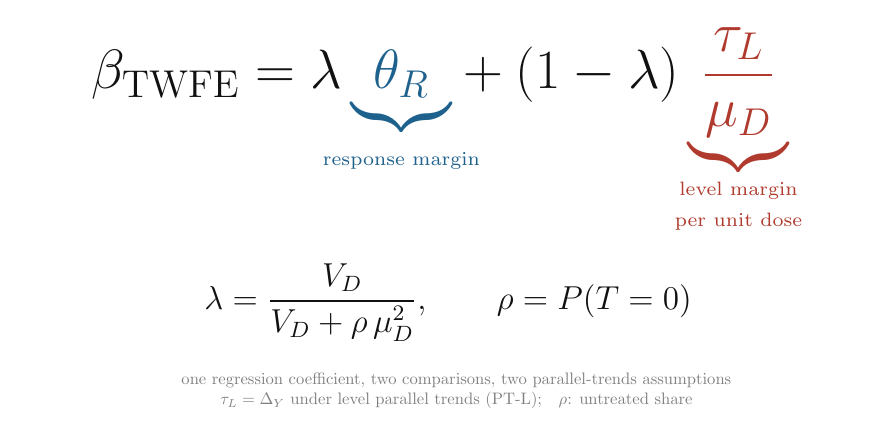
\begin{tikzpicture}[every node/.style={inner sep=0pt, text=ink}]
% 1. dominant line: the two-period TWFE mixture (Theorem 3, eq. (8))
\node[font=\fontsize{20}{24}\selectfont] (main) {%
  $\displaystyle
  \beta_{\mathrm{TWFE}} = \lambda\,
  \textcolor{blue}{\underbrace{\theta_R}_{\mathclap{\lab{response margin}}}}
  + (1-\lambda)\,
  \textcolor{red}{\underbrace{\frac{\tau_L}{\mu_D}}_{\mathclap{\substack{\lab{level margin}\\[0pt] \lab{per unit dose}}}}}
  $};
% 2. the mixing weight (eq. (8)); rho = P(T = 0) is the untreated share
\node[font=\fontsize{12}{14}\selectfont, below=10pt of main, xshift=3pt] (second) {%
  $\displaystyle \lambda = \frac{V_D}{V_D + \rho\,\mu_D^{2}}, \qquad \rho = P(T=0)$};
% 3. grey caption; the tau_L form needs level parallel trends (Assumptions 3 and 4)
\node[font=\fontsize{10}{12.5}\selectfont, text=gray, align=center, below=11pt of second, xshift=3pt, scale=0.6] (cap) {%
  one regression coefficient, two comparisons, two parallel-trends assumptions\\
  $\tau_L = \Delta_Y$ under level parallel trends (PT-L);\quad $\rho$: untreated share};
% widen the bounding box so the zero-width underbrace labels are not clipped by the page edge
\path ([xshift=-8mm]main.west) ([xshift=8mm]main.east);
\end{tikzpicture}
\end{document}
